\section{Evaluation}
\label{sec:eval}

The target of this section is two fold presented in the following two case studies.
First, we demonstrate the severity of conducting \drop attack on the closest peers to the source.
Second, we evaluate the proposed detection mechanism's performance, accuracy and the overhead induced on the system due to the messages exchanged by the different detection steps.
First we describe the simulation framework and the parameters for different simulation configurations. Afterwards the metrics used in both case studies are provided.
Finally, we detail the simulation results and the interpretation in both case studies.

\subsection{Simulation Framework and Parameters}
Our simulation framework is based on OSSim \cite{nguyen2013ossim}. 
OSSim provides a packet level simulator for DONet \cite{zhang2005coolstreaming}, a pull-based online video streaming overlay, which we use in our case studies.
We use the network topology generator GT-ITM \cite{GT} with 1000 peers connected to 400 edge router.

To simulate for the worst case scenarios, we assume malicious peers never leave the overlay once they join.
However, to emulate real life measurements \cite{distribution}, benign peers joining is based on Pareto distribution, while their leaving times is estimated using Lognormal distributions.
Benign peers can rejoin the overlay in a uniform distribution around 10s.

As our proposed attack aims at attacking the overlay once the source starts to send video chunks, we focus on showing both the attack's impact along with the detection mechanism's performance on simulation time of 500s.
The results are calculated over 10 runs for each simulation configuration.

The parameters used in both case studies are provided in Table \ref{tab:parameters}.

\begin{table}[ht]
\center
\caption{Acronyms}
\begin{tabular}{|c|c||c|c|}
\hline

\bf{Var.} & \bf{Desc.}  & \bf{Var.} & \bf{Desc.} \\\hline\hline

mal. headnodes $\eta x$ & $\{5,8,10\}$ & chunk size & 2500B \\\hline
sat. threshold $\satThres$ & $\{0.5,0.7,0.95\}$ & $\treply$ & 10s\\\hline
mal. neighbors $MN$  & $\{0,15,24,70,100\}$ & stream Rate & 400kbps\\\hline
min. responses $\minP$ &  $\{3,4\}$ & buffer size & 30s  \\\hline
det. allowed $\minDR$ & 10 & list size $LS$ & $\{8,10\}$\\\hline
  
\end{tabular}
\label{tab:parameters}
\end{table}

\subsection{Metrics}

Here we define the metrics used throughout the evaluation.
\subsubsection*{Satisfaction $\sat$} which represents the average peer satisfaction level through the whole simulation interval.
\subsubsection*{Avg. Loss} that indicates the avg chunk loss per peer.
\subsubsection*{Detection Overhead $DO$} used to evaluate the detection overhead induced on the system, i.e., the ratio of messages exchanged during due to the detection mechanism over all signaling messages in the system.
\subsubsection*{Benign Ratio per Neighbor List $BRNL$} which measures the ratio of benign peers over all peers in the source's neighbor list.

\subsection{Case 1: \drop Severity}

In this case study, we evaluate the impact of \drop attack on two different network scenarios:  (1) DONet, and (2) DONet+SWAP \cite{nguyen2016swap}, in order to assess the attack's severity when a replacement mechanism for peers is operating.
Note that the attacker's budget is independent from the overlay's size, in fact, the attacker's budget is dependent on the neighbor list size $LS$.
The reason is that as malicious peers target is to occupy the closest peers to the source, the remaining size of the overlay is not a factor on the impact of the \drop attack.
\mn[Hatem]{I'm not entirely sure that the assumption above is always correct, and even if it is correct, shouldn't we back it up with results and numbers, so feel free to remove it.}   

Given the source's neighbor list size $LS=10$, we choose the following combinations for the attackers budget $x={\{\eta x, MN\}}$: $\{10=\{10,0\}\}, \{20=\{5,15\}\}, 77=\{7,70\}\}, 32=\{8,24\}\}$.
In otherwords, $MN=70$ denotes that 7 malicious peers are connected to each of the 10 headnodes.
We start with analyzing the attack's impact on DONet and then we evaluate the resilience of the SWAP mechanism to the attack.

In Figure~\ref{subfig:avg-loss-donet}, the average chunk loss ratio is presented. 
As expected, the average loss is 100\% when $\eta x= LS =10$, which means that the source's $LS$ is utterly saturated with malicious headnodes, i.e., no chunks are transmitted to the rest of the overlay.
Accordingly, the average peer satisfaction in such case is always 0\%. 

For the other cases where $\eta x < 10$; the average loss when the stream starts reaches up to ~82\% for $x=\{7, 70\}$, for $x=\{5, 15\}$ the loss ratio is ~54\% and ~73\% for $x=\{8, 24\}$, as shown in Figure~\ref{subfig:avg-loss-donet}.
% it is noticed that the impact of the attack is significantly successful in dropping the chunk success delivery ratio up to ~82\% once the source starts to send video chunks.
It is inferred that as the value of $\eta x, MN$ increase, benign peers experience remarkable service degradation for a longer time period as a result of having benign peers closer to the source overloaded with requests that they can not completely respond to. 
Nevertheless, the loss ratio decreases once a fraction of benign (headnodes and non-headnodes) peers are able to serve the rest of the overlay.

Figure~\ref{subfig:satisfaction-donet} presents the average peer satisfaction level $\sat$.
As a consequence of experiencing high chunk loss rate, higher values of $\eta x, MN$ result in lower peer satisfaction over time, where benign peers at $x=\{5, 15\}$ restore their satisfaction level at ~340s, which is earlier than at $x=\{7, 70\}$ and $x=\{8, 24\}$.

Now we analyze the attack's impact while SWAP is operating.
While executing SWAP's operations, peers nominate and forward other peers nominations to the source. 
Consequentially, malicious peers abuse the mechanism via nominating other malicious peers at each nomination round. 
Moreover, malicious peers connected to benign headnodes are eventually nominated to the source and thus, results in occupying the sources $LS$.

As shown in Figure~\ref{subfig:avg-loss-donet}, comparing the same values at $x=\{5, 15\}$ for both DONet and SWAP show that the impact of the attack when SWAP is operating is more significant.
Before the source's $LS$ is saturated with malicious peers at $t=80s$, the average loss is in fact decreasing, However, afterwards the the average chunk loss increases up to ~97\% as a result of more malicious peers being promoted as headnodes, which in turn decreases the fraction of reachable chunks to benign peers.
For the same reason, the satisfaction level of benign peers eventually decreases to ~6\%, which highlights the unsuitability of SWAP against our proposed attack.

\begin{figure}[t!]
\centering

  \mbox{\subfloat[Avg. loss]{\label{subfig:avg-loss-donet}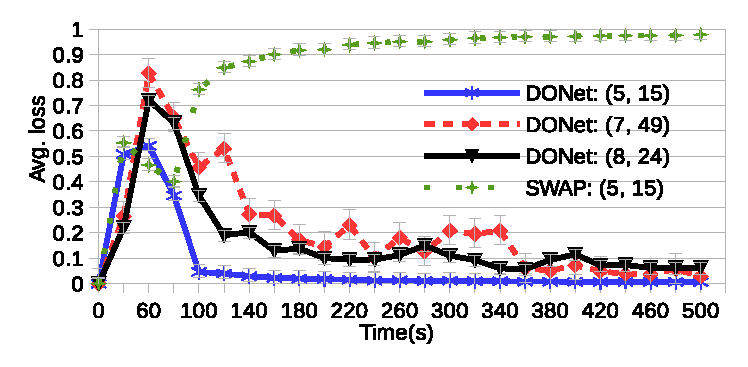
\includegraphics[width=8.4cm,height=3.5cm]{./Figures/avg-loss-donet.eps}}}
 
  \mbox{\subfloat[Avg. peer satisfaction]{\label{subfig:satisfaction-donet}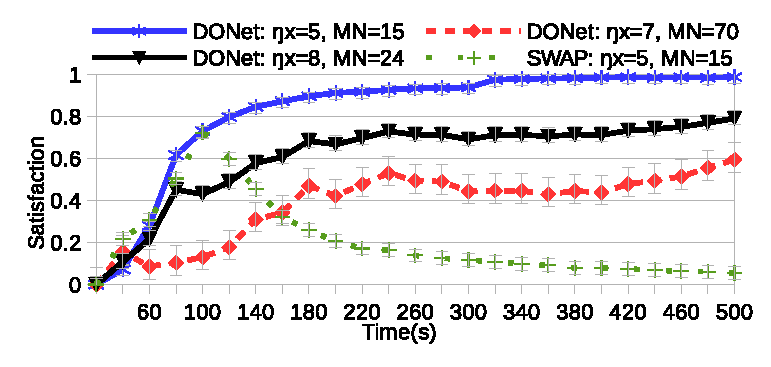
\includegraphics[width=8.4cm,height=3.5cm]{./Figures/satisfaction-donet.eps}}}
%   \mbox{\subfloat[Avg. loss]{\label{subfig:avg-loss-donet}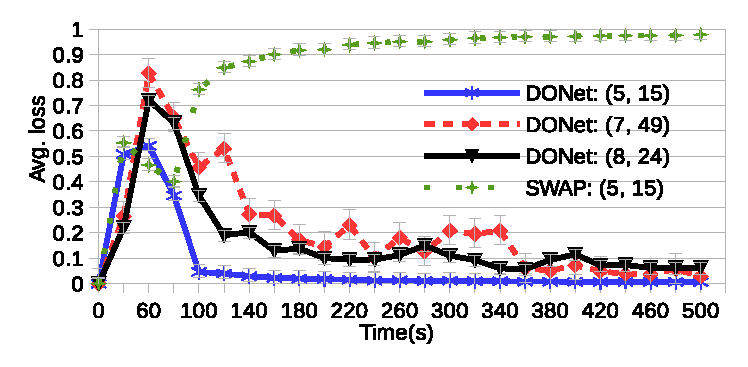
\includegraphics[width=3.7cm,height=2.5cm]{./Figures/avg-loss-donet.eps}} \subfloat[Avg. peer satisfaction]{\label{subfig:satisfaction-donet}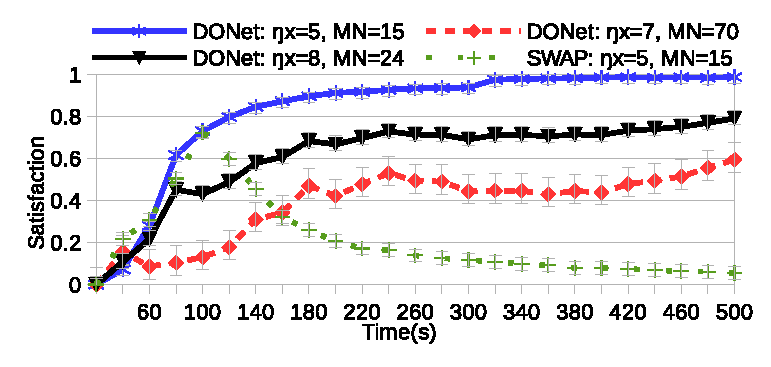
\includegraphics[width=3.7cm,height=2.5cm]{./Figures/satisfaction-donet.eps}}} 
  \caption{Attack's impact on DONet}
  \label{fig:attack-results}
  \end{figure}


\subsection{Case 2: Detection Mechanism Performance}

\begin{figure}[t!]
\centering

  \mbox{\subfloat[Avg. BRNL]{\label{subfig:BRNL}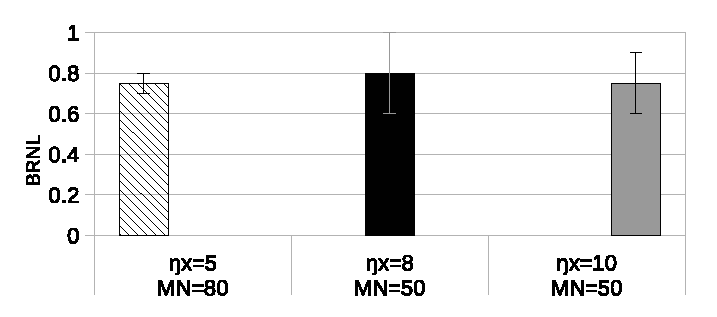
\includegraphics[width=8.4cm,height=3.5cm]{./Figures/det-BRNL.eps}}}
 
  \mbox{\subfloat[Avg. peer satisfaction]{\label{subfig:det-sat}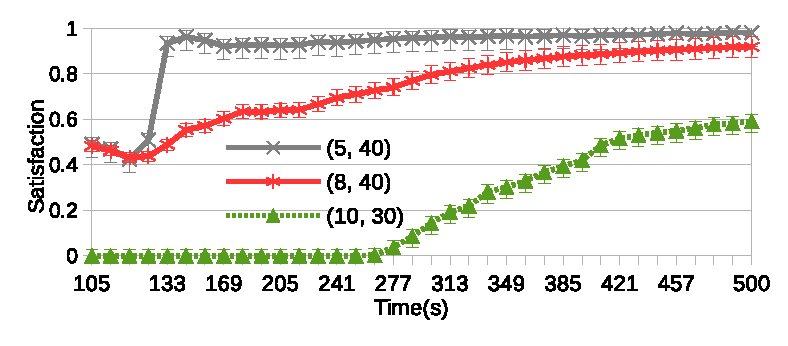
\includegraphics[width=8.4cm,height=3.5cm]{./Figures/det-sat.eps}}}
%   \mbox{\subfloat[Avg. loss]{\label{subfig:avg-loss-donet}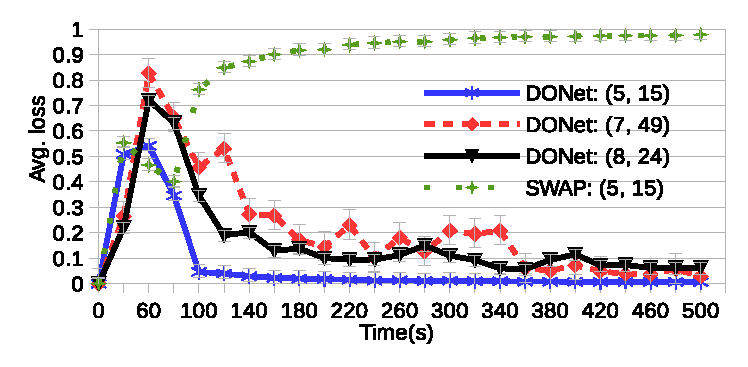
\includegraphics[width=3.7cm,height=2.5cm]{./Figures/avg-loss-donet.eps}} \subfloat[Avg. peer satisfaction]{\label{subfig:satisfaction-donet}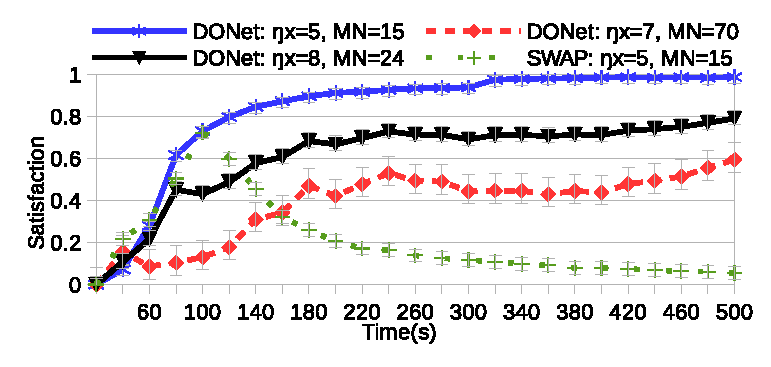
\includegraphics[width=3.7cm,height=2.5cm]{./Figures/satisfaction-donet.eps}}} 
  \caption{Detection mechanism performance}
  \label{fig:detection-results}
  \end{figure}


% \subsubsection{Summary of the results}
% 
% As a summary, for DONet, when the source's neighbor list is fully saturated with malicious peers, $IL$ is at ~100\%.
% Nevertheless, for smaller values of $Hx$, the attack's impact is still significantly high for a long period of time given the intolerability of such networks to such high delays.
% In fact, having only $Hx=\alpha$ without using $MN$ is sufficient for the attacker to completely isolate and thus, prevent the source from delivering any stream chunks.
% 
% For the SWAP case study, it is noticed that even with low values of $Hx$, after a certain swapping period, malicious peers manage to fully occupy the source's list and hence, $IL$ eventually reaches to ~100\%.
% This denotes that, the number of neighbors $MN$ is a major factor in the case of SWAP.
% Moreover, through an efficient distribution of the attacker's budget $x$, i.e., $Hx$ and $MN$, the attacker can decide whether to cause higher damage to the stream at the initialization time and then allow the network to eventually recover later on, or to allow the stream to reach to benign peers at earlier time phase till totally cutting the flow once $Hx=\alpha$ at some point.